%----------------------------------------------------------------------------------------
%   PACKAGES AND THEMES
%----------------------------------------------------------------------------------------

\documentclass[aspectratio=169]{beamer}

\mode<presentation> {

% The Beamer class comes with a number of default slide themes
% which change the colors and layouts of slides. Below this is a list
% of all the themes, uncomment each in turn to see what they look like.

%\usetheme{default}
%\usetheme{AnnArbor}
%\usetheme{Antibes}
%\usetheme{Bergen}
%\usetheme{Berkeley}
%\usetheme{Berlin}
%\usetheme{Boadilla}
%\usetheme{CambridgeUS}
%\usetheme{Copenhagen}
%\usetheme{Darmstadt}
%%%%%%%\usetheme{Dresden}
%\usetheme{Frankfurt}
%\usetheme{Goettingen}
%\usetheme{Hannover}
%\usetheme{Ilmenau}
%\usetheme{JuanLesPins}
\usetheme{Luebeck}
%\usetheme{Madrid} 
%\usetheme{Malmoe}
%\usetheme{Marburg}
%\usetheme{Montpellier}
%\usetheme{PaloAlto}
%\usetheme{Pittsburgh}
%\usetheme{Rochester}
%\usetheme{Singapore}
%\usetheme{Szeged}
%\usetheme{Warsaw}

% As well as themes, the Beamer class has a number of color themes
% for any slide theme. Uncomment each of these in turn to see how it
% changes the colors of your current slide theme.

%\usecolortheme{albatross}
%%%%%\usecolortheme{beaver}
%\usecolortheme{beetle}
%\usecolortheme{crane}
%\usecolortheme{dolphin}
%\usecolortheme{dove}
%\usecolortheme{fly}
%\usecolortheme{lily}
%\usecolortheme{orchid}
%\usecolortheme{rose}
%\usecolortheme{seagull}
%\usecolortheme{seahorse}
%\usecolortheme{whale}
%\usecolortheme{wolverine}
\usecolortheme{default}

%\setbeamertemplate{footline} % To remove the footer line in all slides uncomment this line
%\setbeamertemplate{footline}[page number] % To replace the footer line in all slides with a simple slide count uncomment this line

%\setbeamertemplate{navigation symbols}{} % To remove the navigation symbols from the bottom of all slides uncomment this line
}


\addtobeamertemplate{navigation symbols}{}{%
    \usebeamerfont{footline}%
    \usebeamercolor[fg]{footline}%
    \hspace{1em}%
    \insertframenumber/\inserttotalframenumber
}



\usepackage{graphicx} % Allows including images
\usepackage{booktabs} % Allows the use of \toprule, \midrule and \bottomrule in tables
\usepackage[utf8]{inputenc}

\usepackage{ragged2e}
\usepackage{lmodern}
\usepackage{array}
\usepackage[normalem]{ulem}
\usepackage{microtype}

\usepackage{graphicx}
\graphicspath{ {images/} }

\setbeamerfont{footnote}{size=\tiny}

%----------------------------------------------------------------------------------------
%   TITLE PAGE
%----------------------------------------------------------------------------------------


\title[Protocolos de Experimentação]{Planejamento de Protocolos de Experimentação em Engenharia
de Software usando \textit{Business Process Model}} 
% The short title appears at the bottom of every slide, the full title is only on the title page

\author[Leandro Ungari Cayres]{Leandro Ungari Cayres \\Orientador: Prof. Dr. Rogério Eduardo Garcia} % Your name

\institute[UNESP] % Your institution as it will appear on the bottom of every slide, may be shorthand to save space
{
Universidade Estadual Paulista \\ % Your institution for the title page
\medskip
\textit{leandroungari@gmail.com} % Your email address
}
\date{17 de Agosto de 2017} % Date, can be changed to a custom date

\begin{document}

\begin{frame}
\titlepage % Print the title page as the first slide
\end{frame}

%----------------------------------------------------------------------------------------
%   PRESENTATION SLIDES
%----------------------------------------------------------------------------------------
\begin{frame}
\frametitle{Visão Geral}
\tableofcontents
\end{frame}

%==================
\begin{frame}
\frametitle{Problemática}
\justifying

\begin{columns}

\begin{column}{0.5\textwidth}
\begin{itemize}
\item Processo Experimental
\end{itemize}
\end{column}

\begin{column}{0.5\textwidth}
\begin{figure}
\centering

\includegraphics[scale=0.35]{images/experimento.jpg}
\end{figure}
\end{column}
\end{columns}




\end{frame}

%==================
\begin{frame}
\frametitle{Problemática}
\justifying

\begin{columns}

\begin{column}{0.5\textwidth}
\begin{itemize}
\item Processo Experimental
\item Pacote de Laboratório
\end{itemize}
\end{column}

\begin{column}{0.5\textwidth}
\begin{figure}
\centering
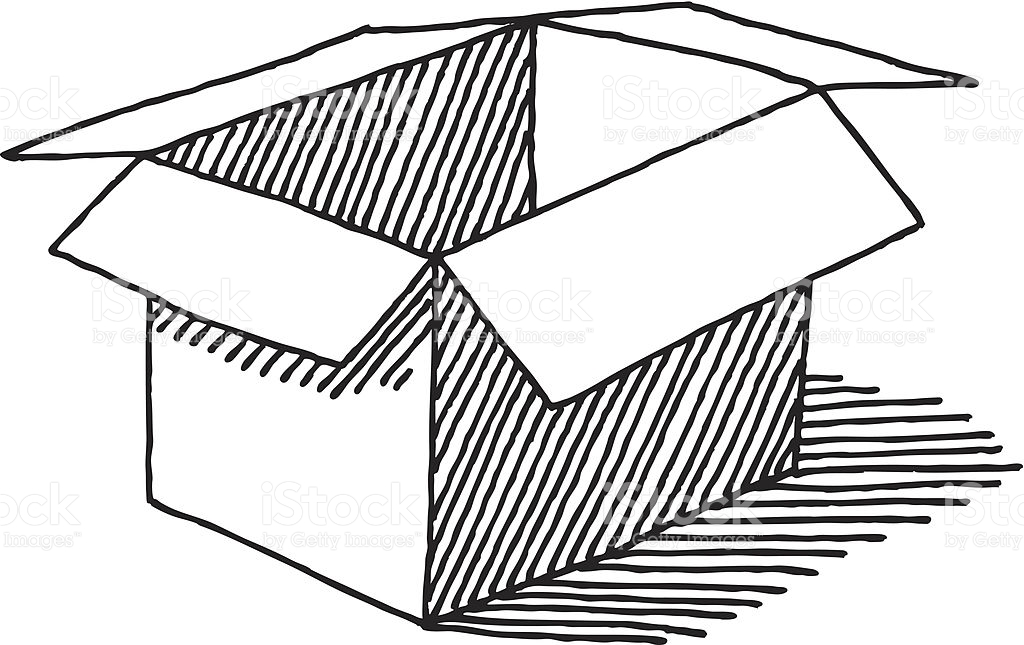
\includegraphics[scale=0.2]{images/box.jpg}
\end{figure}
\end{column}
\end{columns}

\end{frame}

%==================
\begin{frame}
\frametitle{Problemática}
\justifying

\begin{columns}

\begin{column}{0.5\textwidth}

\begin{itemize}
\item Processo Experimental
\item Pacote de Laboratório
\item Protocolo de Experimentação
\end{itemize}

\end{column}

\begin{column}{0.5\textwidth}
\begin{figure}
\centering

\includegraphics[scale=0.2]{images/paper.jpg}
\end{figure}
\end{column}
\end{columns}



\end{frame}

%==================
\begin{frame}
\frametitle{Objetivos Gerais}
\justifying

\begin{itemize}
\item Prover uma interface capaz de representar visualmente o protocolo de um experimento, através da notação BPM:
\end{itemize}
\end{frame}

%==================
\begin{frame}
\frametitle{Objetivos Gerais}
\justifying

\begin{itemize}
\item Prover uma interface capaz de representar visualmente o protocolo de um experimento, através da notação BPM:
\\~\\
\begin{enumerate}
\item Possibilitar ao experimentador a possibilidade de planejamento e construção do protocolo de experimentação.
\end{enumerate}
\end{itemize}
\end{frame}

%==================
\begin{frame}
\frametitle{Objetivos Gerais}
\justifying

\begin{itemize}
\item Prover uma interface capaz de representar visualmente o protocolo de um experimento, através da notação BPM:
\\~\\
\begin{enumerate}
\item Possibilitar ao experimentador a possibilidade de planejamento e construção do protocolo de experimentação.
\item Viabilizar a visualização do protocolo de experimentação contido em um pacote de laboratório.
\end{enumerate}
\end{itemize}
\end{frame}

\begin{frame}
\frametitle{Objetivos Específicos}
\justifying
\begin{itemize}
\item Aplicação de modificações na camada de apresentação da ferramenta \textit{OntoExpTool}, incorporando o modelo gráfico a esta, e consequentemente, as alterações necessárias na camada de controle.
\end{itemize}

\end{frame}

\begin{frame}
\frametitle{Objetivos Específicos}
\justifying

\begin{itemize}
\item Aplicação de modificações na camada de apresentação da ferramenta \textit{OntoExpTool}, incorporando o modelo gráfico a esta, e consequentemente, as alterações necessárias na camada de controle.
\\~\\
\item Construção de um sistema de software que possibilite a concepção e troca de pacotes de laboratório, para a condução de experimentos controlados.


\end{itemize}


\end{frame}

%-----------------------------------------------
\section{Engenharia de Software Experimental}
%==================
\begin{frame}
\frametitle{Engenharia de Software Experimental}
\justifying

\begin{itemize}
\item Busca medir e avaliar modelos e tecnologias
\end{itemize}

\end{frame}

%==================
\begin{frame}
\frametitle{Engenharia de Software Experimental}
\justifying

\begin{itemize}
\item Busca medir e avaliar modelos e tecnologias
\item Corpo de conhecimento
\end{itemize}

\end{frame}

%==================
\begin{frame}
\frametitle{Engenharia de Software Experimental}
\justifying

\begin{itemize}
\item Busca medir e avaliar modelos e tecnologias
\item Corpo de conhecimento
\item Estudo isolado
\end{itemize}

\end{frame}

%==================
\begin{frame}
\frametitle{Engenharia de Software Experimental}
\justifying

\begin{itemize}
\item Busca medir e avaliar modelos e tecnologias
\item \sout{Corpo de conhecimento}
\item Estudo isolado
\end{itemize}

\end{frame}

%==================
\begin{frame}
\frametitle{Engenharia de Software Experimental}
\justifying

\begin{itemize}
\item Busca medir e avaliar modelos e tecnologias
\item \sout{Corpo de conhecimento}
\item Estudo isolado
\item Estudos Experimentais
\end{itemize}

\end{frame}

%==================
\begin{frame}
\frametitle{Estudos Experimentais}
\justifying

Os Estudos Experimentais atuam como ferramentas para obtenção dos dados necessários através de todo o processo de desenvolvimento de software, almejando resultados objetivos e significativos de forma a alcançar melhorias no processo.

\end{frame}

%==================
\begin{frame}
\frametitle{Estudos Experimentais}
\justifying

Segundo Wohlin et al.(2012), tais estudos podem ser divididos nas seguintes categorias: \\~\\
\begin{itemize}
\item Pesquisa de Opinião
\item Estudo de Caso
\item Experimento Controlado
\end{itemize}

\end{frame}

%==================
\begin{frame}
\frametitle{Estudos Experimentais}
\justifying

Segundo Wohlin et al.(2012), tais estudos podem ser divididos nas seguintes categorias: \\~\\
\begin{itemize}
\item Pesquisa de Opinião
\item Estudo de Caso
\item \underline{Experimento Controlado}
\end{itemize}

\end{frame}

%==================
\begin{frame}

\begin{figure}
\centering
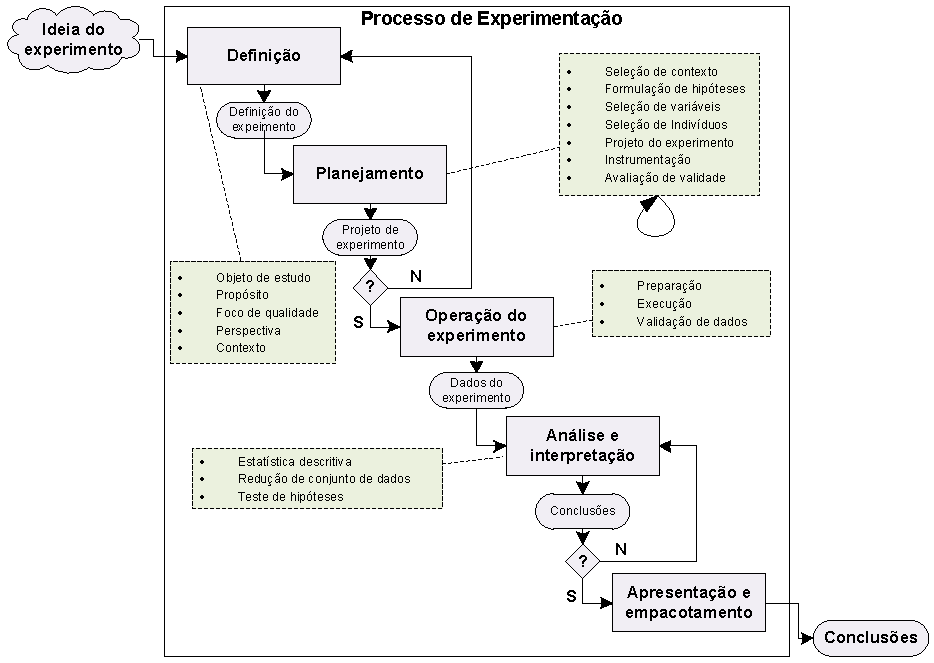
\includegraphics[scale=0.5]{images/experimentacao.pdf}
\caption{Processo de Experimentação~\cite{wohlin}.}
\label{image:processo}
\end{figure}

\end{frame}


%==================
\begin{frame}
\justifying

\begin{figure}
\centering
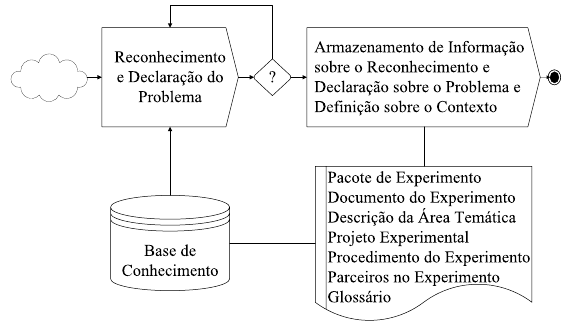
\includegraphics[scale=0.5]{images/definicao.png}
\caption{Fase de Definição~\cite{Garcia06}.}
\label{image:definicao}
\end{figure}

\end{frame}

%==================
\begin{frame}
\justifying

\begin{figure}
\centering
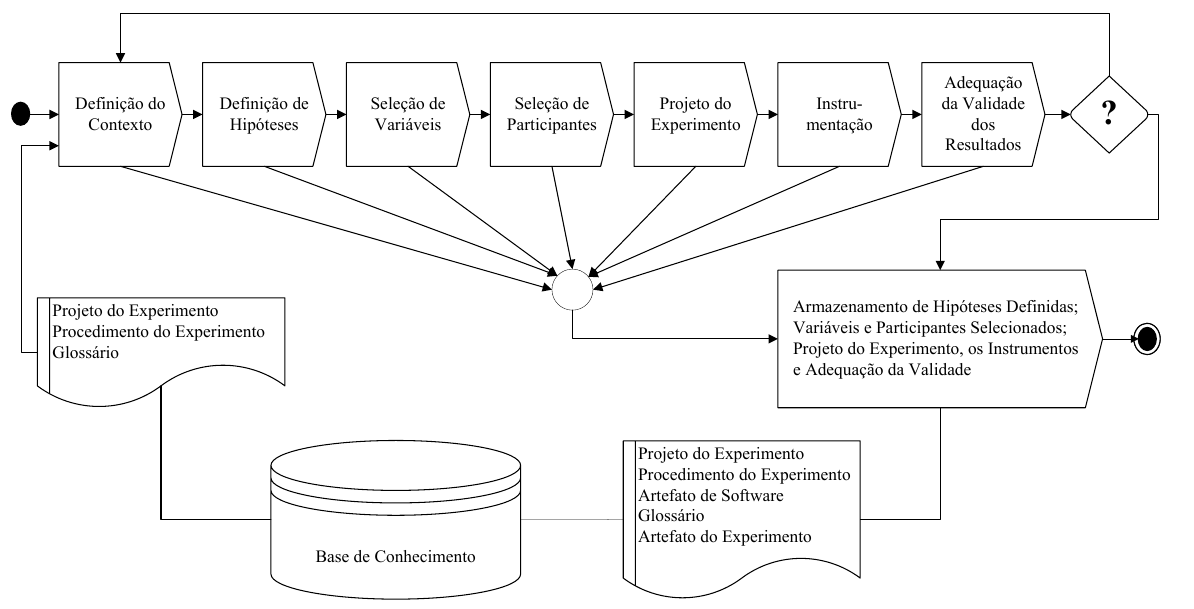
\includegraphics[scale=0.3]{images/planejamento.png}
\caption{Fase de Planejamento~\cite{Garcia06}.}
\label{image:planejamento}
\end{figure}

\end{frame}

%==================
\begin{frame}
\justifying

\begin{figure}
\centering
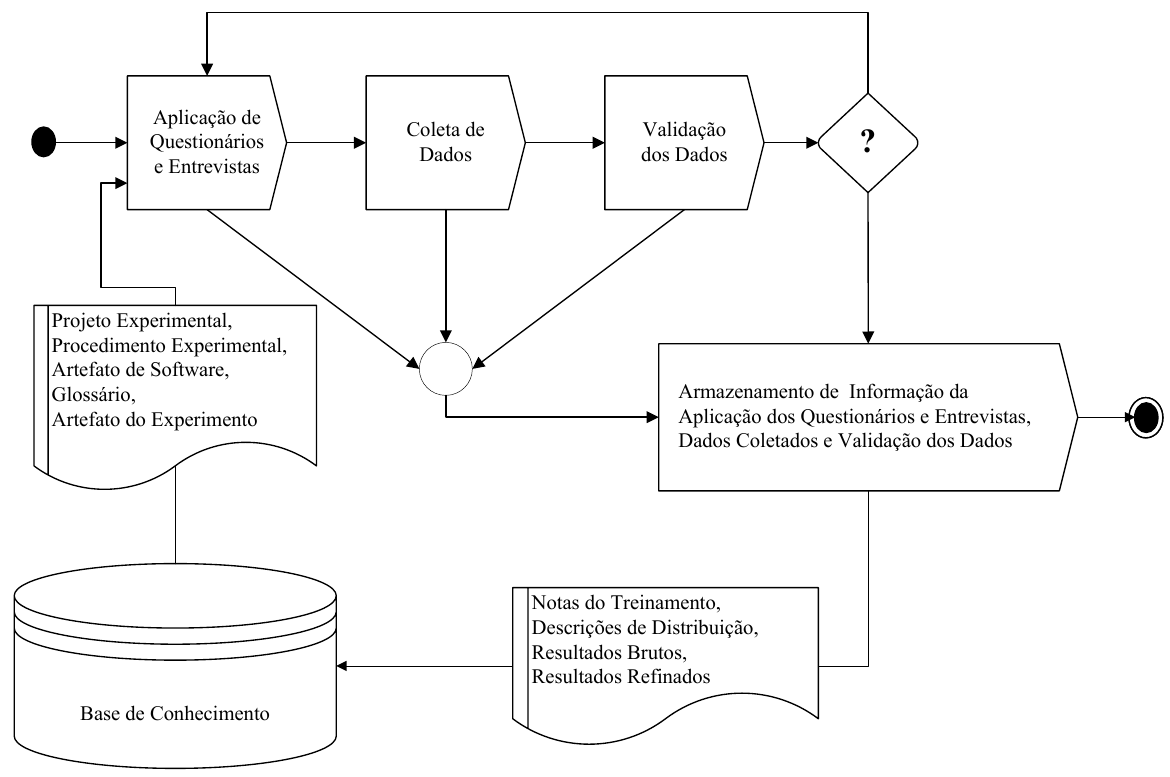
\includegraphics[scale=0.25]{images/operacao.png}
\caption{Fase de Operação~\cite{Garcia06}.}
\label{image:operacao}
\end{figure}

\end{frame}

%==================
\begin{frame}
\justifying

\begin{figure}
\centering
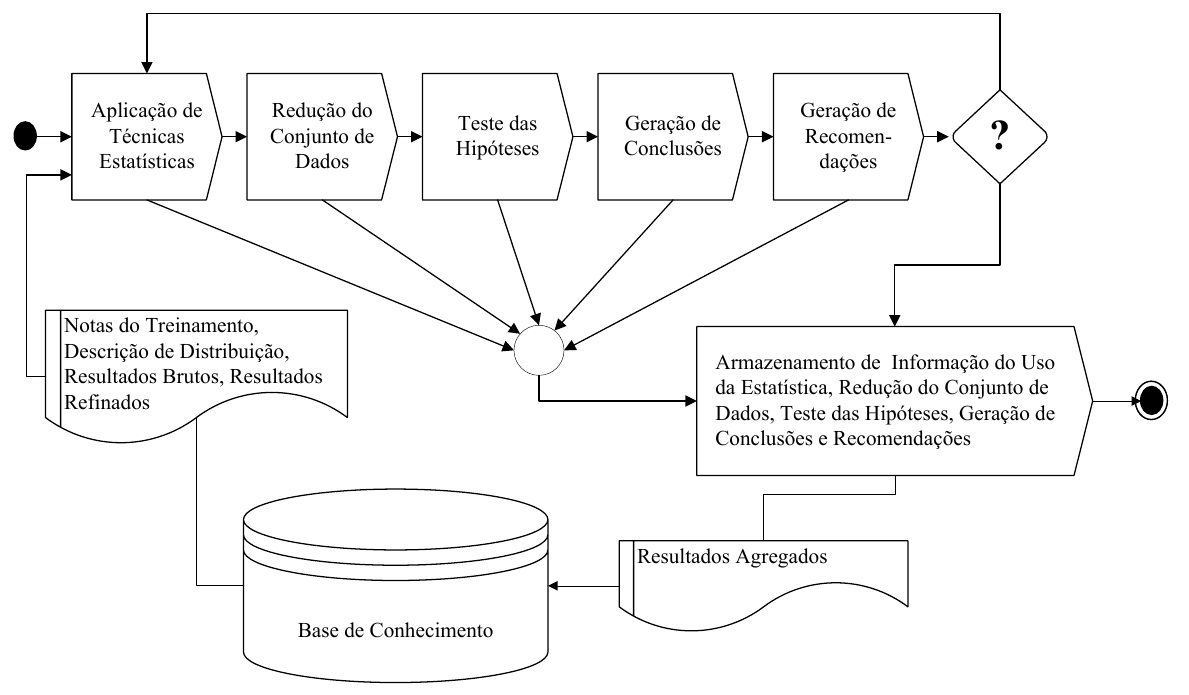
\includegraphics[scale=0.25]{images/analise.png}
\caption{Fase de Análise e Interpretação~\cite{Garcia06}.}
\label{image:analise}
\end{figure}

\end{frame}

%==================
\begin{frame}
\frametitle{Processo de Replicação}
\justifying
Segundo Basili et al. (1999), a construção de um corpo de conhecimento em Engenharia de Software requer a execução de famílias de experimentos e adoção de um conjunto de princípios unificados que permita \underline{combinar e generalizar} resultados.
\end{frame}

%==================
\begin{frame}
\justifying

\begin{figure}
\centering
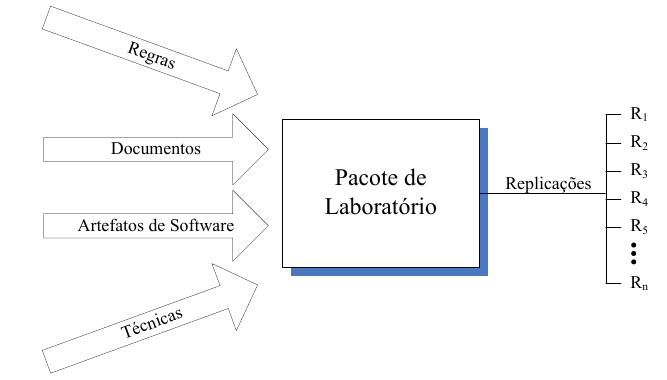
\includegraphics[scale=0.45]{images/replicacao.png}
\caption{Processo de Replicação~\cite{Garcia06}.}
\label{image:replicacao}
\end{figure}

\end{frame}

%------------------------------------------------
\section{Pacotes de Laboratório}

\begin{frame}
\frametitle{Pacote de Laboratório}
\justifying
Diversas pesquisas, técnicas e ferramentas são desenvolvidos para validar teses ou otimizar soluções, porém recursos ou informações isoladas não formam um \underline{corpo de conhecimento} consistente, faz-se necessário \underline{compartilhá-los} entre os grupos de pesquisa por meio do uso de \underline{pacotes de laboratório}.

\end{frame}

\begin{frame}
\frametitle{\textit{ExperOntology}}
\justifying
A \textit{ExperOntology} é apresentada como uma ontologia para Engenharia de Software Experimental, baseando-se no conhecimento de pesquisadores e na experiência em condução de experimentos controlados, principalmente na avaliação das técnicas V\&V (Validação e Verificação).
\end{frame}

%==================
\begin{frame}
\justifying

\begin{figure}
\centering
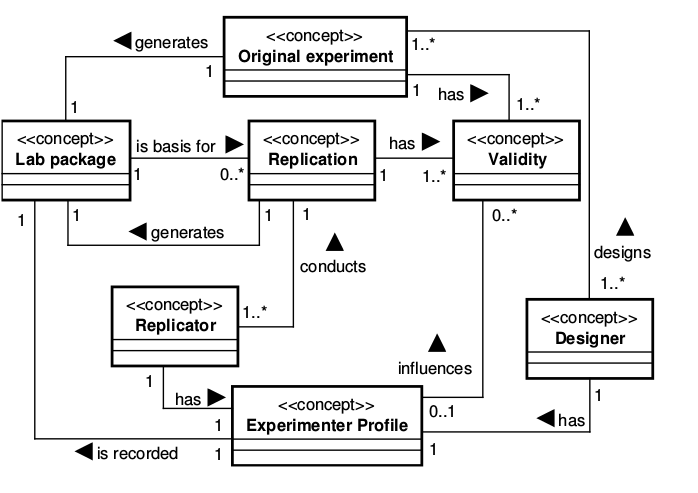
\includegraphics[scale=0.4]{images/controlados.png}
\caption{Ontologia para Experimentos Controlados~\cite{Garcia08}.}
\label{image:controlados}
\end{figure}


\end{frame}

%==================
\begin{frame}
\justifying

\begin{figure}
\centering
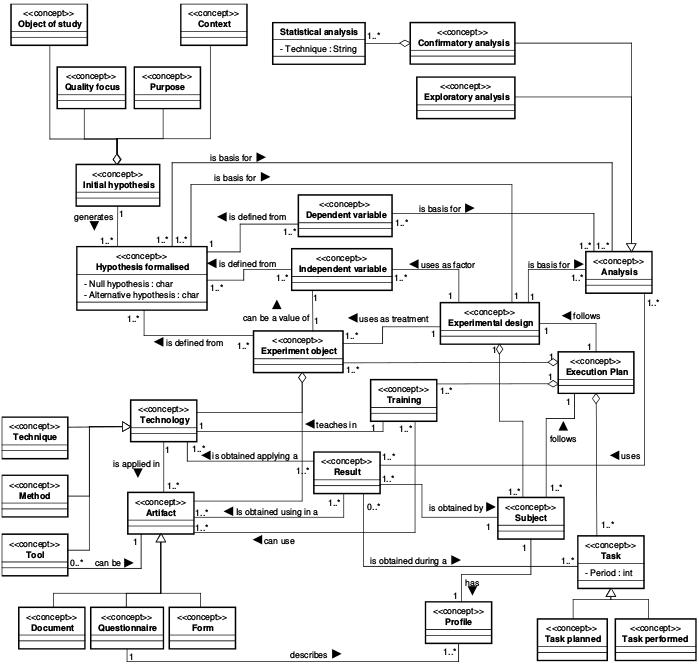
\includegraphics[scale=0.33]{images/onto.png}
\caption{Ontologia para Pacotes de Laboratório~\cite{Garcia08}.}
\label{image:ontolgia}
\end{figure}

\end{frame}

\begin{frame}
\frametitle{Modelo Relacional}
\justifying

O modelo relacional de dados tem sido utilizado em larga escala desde a sua criação. Este modelo tem como característica a utilização de tabelas e tuplas para o armazenamento de dados, assim como o uso de chaves primárias para garantia de unicidade (identificação única de elementos de dados) (Brito, 2010).

\end{frame}

\begin{frame}
\frametitle{Modelo Relacional}
\justifying
\begin{figure}
\centering
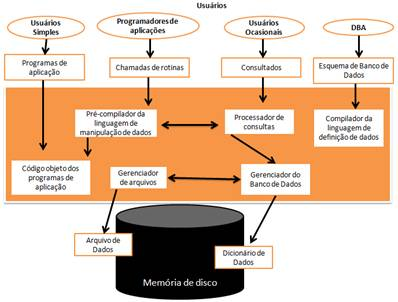
\includegraphics[scale=.6]{images/sgbd.jpg}
\caption{Arquitetura de um SGBD.}
\label{image:sgbd}

\end{figure}


\end{frame}

\begin{frame}
\frametitle{Modelo Não-Relacional}
\justifying
Como alternativa, há soluções tecnológicas alternativas que priorizam flexibilidade quanto ao armazenamento, desse modo, não empregam regras presentes no modelo relacional tradicional.\\~\\
\begin{itemize}
\item Orientado a Colunas (\textit{Column})
\end{itemize}
\end{frame}

\begin{frame}
\frametitle{Modelo Não-Relacional}
\justifying
Como alternativa, há soluções tecnológicas alternativas que priorizam flexibilidade quanto ao armazenamento, desse modo, não empregam regras presentes no modelo relacional tradicional.\\~\\
\begin{itemize}
\item Orientado a Colunas (\textit{Column})
\item Armazenamento em Documentos (\textit{Documents})
\end{itemize}
\end{frame}


\begin{frame}
\frametitle{Modelo Não-Relacional}
\justifying
Como alternativa, existem soluções tecnológicas alternativas que priorizam flexibilidade quanto ao armazenamento, desse modo, não empregam regras presentes no modelo relacional tradicional.\\~\\
\begin{itemize}
\item Orientado a Colunas (\textit{Column})
\item Armazenamento em Documentos (\textit{Documents})
\item Armazenamento Chave/Valor (\textit{Key/Value})
\end{itemize}
\end{frame}

\begin{frame}
\frametitle{Modelo Não-Relacional}
\justifying
Como alternativa, há soluções tecnológicas alternativas que priorizam flexibilidade quanto ao armazenamento, desse modo, não empregam regras presentes no modelo relacional tradicional.\\~\\
\begin{itemize}
\item Orientado a Colunas (\textit{Column})
\item Armazenamento em Documentos (\textit{Documents})
\item Armazenamento Chave/Valor (\textit{Key/Value})
\item Armazenamento em Grafos (\textit{Graph})
\end{itemize}

\end{frame}

\begin{frame}
\frametitle{Modelo Não-Relacional}
\justifying
Como alternativa, há soluções tecnológicas alternativas que priorizam flexibilidade quanto ao armazenamento, desse modo, não empregam regras presentes no modelo relacional tradicional.\\~\\
\begin{itemize}
\item Orientado a Colunas (\textit{Column})
\item \underline{Armazenamento em Documentos} (\textit{Documents})
\item Armazenamento Chave/Valor (\textit{Key/Value})
\item Armazenamento em Grafos (\textit{Graph})
\end{itemize}

\end{frame}

%------------------------------------------------
\section{Modelagem de Processo de Negócio}
%==================
\begin{frame}
\frametitle{Modelagem de Processo de Negócio}
\justifying
\begin{columns}

\begin{column}{0.5\textwidth}
Um processo de negócio é descrito por um ou mais procedimentos que, de modo conjunto, focam a realização de um objetivo de negócio.
\end{column}

\begin{column}{0.5\textwidth}
\begin{figure}
\centering
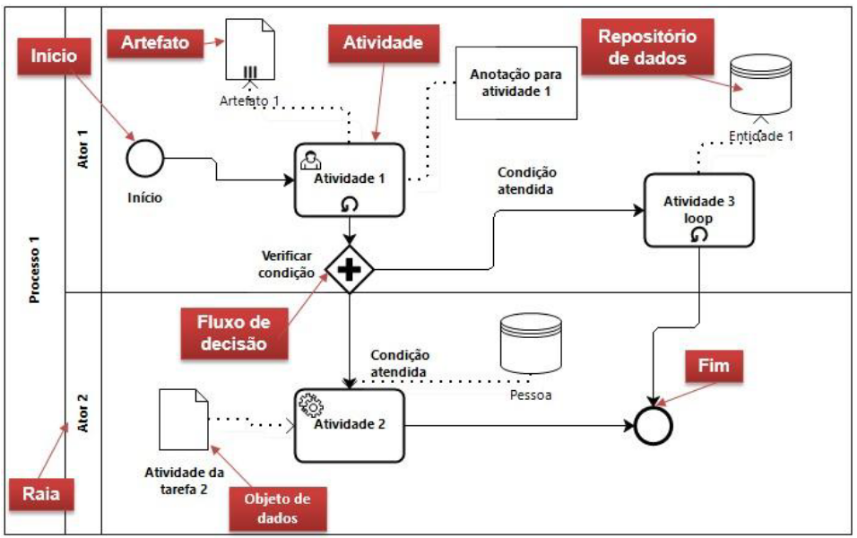
\includegraphics[scale=0.25]{images/diagrama.png}
\caption{Exemplo de modelo de processo de negócio.}
\label{image:exemplo}
\end{figure}
\end{column}
\end{columns}

\end{frame}

\begin{frame}
\frametitle{Modelagem de Processo de Negócio}
\justifying

Um processo de negócio pode ser modelado através das seguintes perspectivas:
\begin{itemize}
\item Controle de Fluxo
\item Dados
\item Organizacional
\item Tratamento de Exceções
\end{itemize}

\end{frame}

\begin{frame}
\frametitle{\textit{Business Process Modeling and Notation}}

\begin{columns}
\begin{column}{0.5\textwidth}

A especificação da notação BPMN foi elaborada e lançada em 2004 pelo Instituto de Gerenciamento de Processos de Negócio (BPMI - \textit{Business Process Management Institute}).\\~\\

\end{column}

\begin{column}{0.5\textwidth}
\begin{figure}
\centering

\includegraphics[scale=0.22]{images/logo-bpmn.png}
\caption{Business Process Modeling and Notation~\cite{OMG}.}
\label{image:logo-bpmn}
\end{figure}
\end{column}
\end{columns}

\end{frame}

\begin{frame}
\frametitle{\textit{Business Process Modeling and Notation}}
\justifying
Posteriormente, a notação BPMN foi adotada pelo Consórcio OMG (\textit{Object Management Group}) como o padrão para modelagem de processos. Após a padronização, foram lançadas algumas versões subsequentes, atualmente encontrando-se em sua segunda versão.

\begin{figure}
\centering

\includegraphics[scale=0.28]{images/logo.jpg}
\caption{Object Management Group~\cite{OMG}.}
\label{image:logo-omg}
\end{figure}

\end{frame}

\begin{frame}
\frametitle{\textit{Business Process Modeling and Notation}}
\justifying

A especificação completa da atual versão divide seus elementos em quatro categorias básicas:

\begin{itemize}
\item Objetos de fluxo (\textit{Flow Objects})
\item Objetos de conexão (\textit{Connecting Objects})
\item Vias (\textit{Swimlanes})
\item Artefatos (\textit{Artifacts})
\end{itemize}


\end{frame}

\begin{frame}
\frametitle{\textit{Business Process Modeling and Notation}}
\justifying

\begin{figure}
\centering
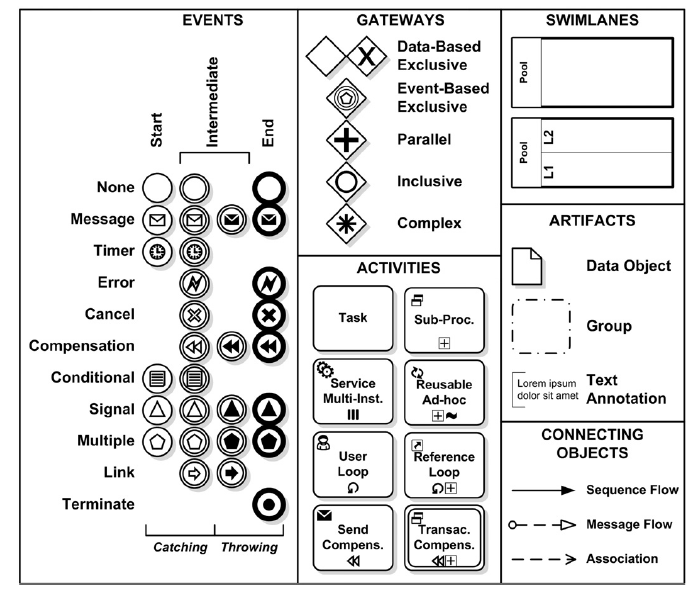
\includegraphics[scale=0.32]{images/elementos.png}
\caption{Conjunto de elementos que compõem a versão BPMN 2.0~\cite{OMG}.}
\label{image:bpmn}
\end{figure}

\end{frame}

%==================
\begin{frame}
\frametitle{Exemplo}
\justifying

\begin{figure}
\centering
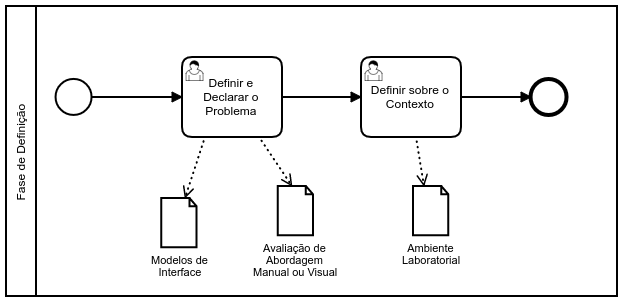
\includegraphics[scale=0.32]{images/modelo-definicao.png}
\caption{Fase de Definição -- adaptado de~\cite{martins}.}
\label{image:fase-definicao}
\end{figure}


\end{frame}

%==================
\begin{frame}
\frametitle{Exemplo}
\justifying

\begin{figure}
\centering
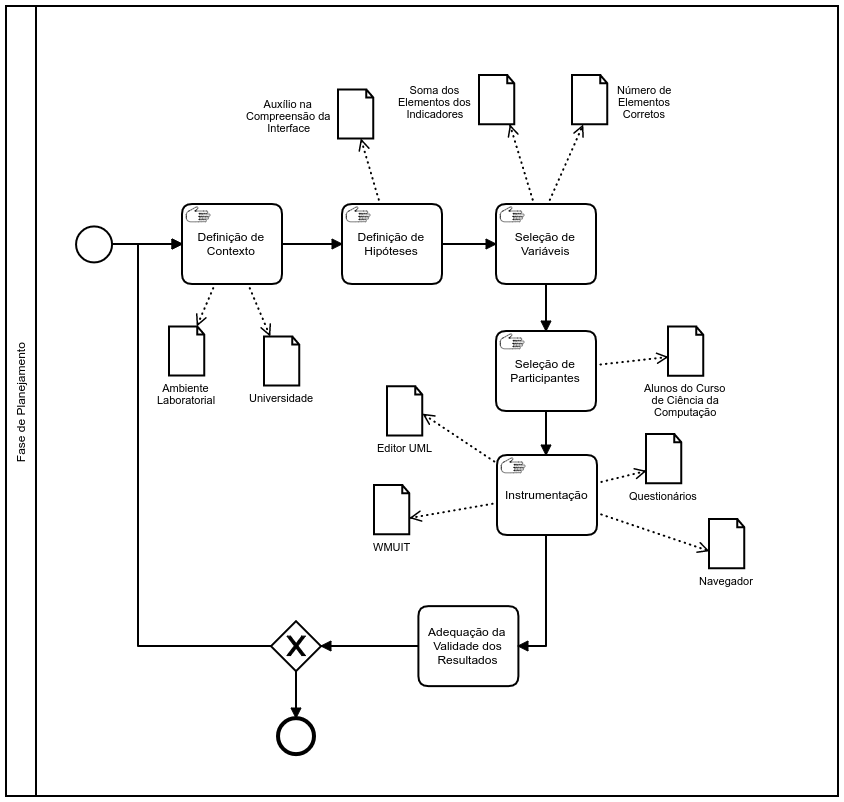
\includegraphics[scale=0.17]{images/modelo-planejamento.png}
\caption{Fase de Planejamento -- adaptado de~\cite{martins}.}
\label{image:fase-planejamento}
\end{figure}


\end{frame}

%==================
\begin{frame}
\frametitle{Exemplo}
\justifying

\begin{figure}
\centering
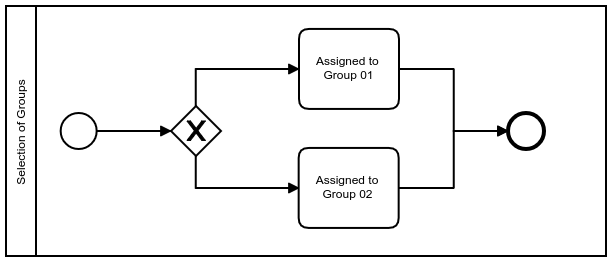
\includegraphics[scale=0.32]{images/selecao.png}
\caption{Fase de Operação - Seleção dos Grupos -- adaptado de~\cite{martins}.}
\label{image:selecao-grupos}
\end{figure}

\end{frame}

%==================
\begin{frame}
\frametitle{Exemplo}
\justifying

\begin{figure}
\centering
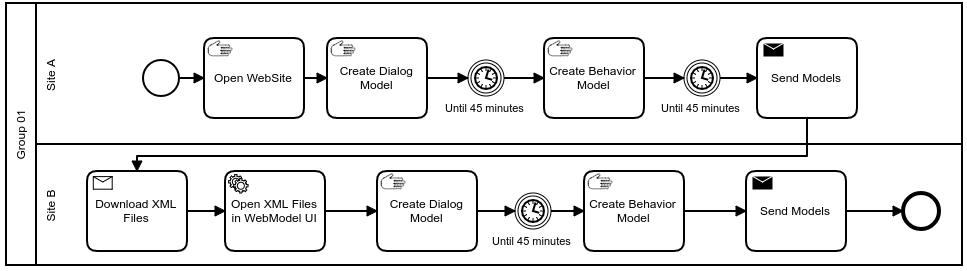
\includegraphics[scale=0.32]{images/grupo01.png}
\caption{Fase de Operação - Atividades do Grupo 01 -- adaptado de~\cite{martins}.}
\label{image:grupo01}
\end{figure}

\end{frame}

%==================
\begin{frame}
\frametitle{Exemplo}
\justifying

\begin{figure}
\centering
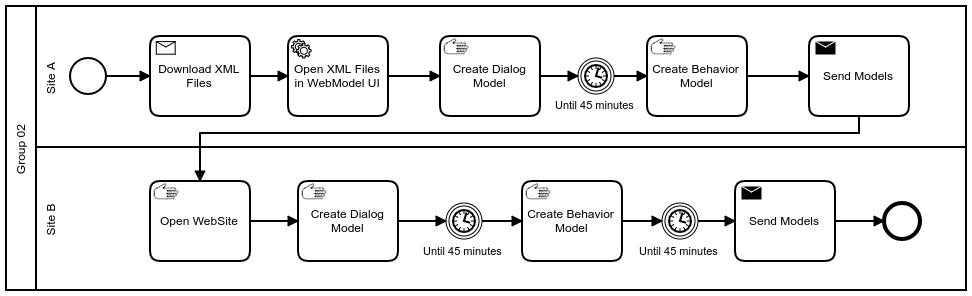
\includegraphics[scale=0.3]{images/grupo02.png}
\caption{Fase de Operação - Atividades do Grupo 02 -- adaptado de~\cite{martins}.}
\label{image:grupo02}
\end{figure}


\end{frame}


%==================
\begin{frame}
\frametitle{Exemplo}
\justifying

\begin{figure}
\centering
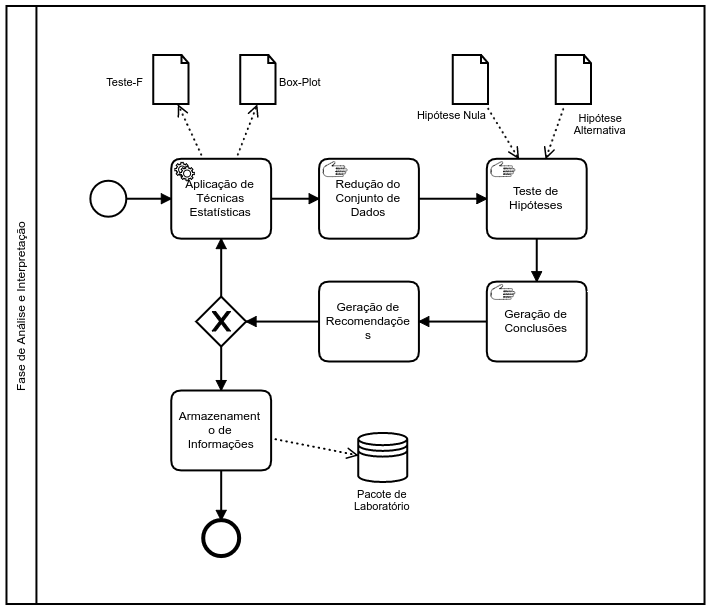
\includegraphics[scale=0.23]{images/modelo-analise.png}
\caption{Fase de Análise e Interpretação~\cite{martins}.}
\label{image:fase-analise}
\end{figure}


\end{frame}

\begin{frame}
\frametitle{Considerações Finais}
\justifying
É possível notar diversos relatos na literatura indicando dificuldades no processo de replicação de estudos experimentais, muitos destes referentes a inexistência de informações relativas ao protocolo de experimentação em pacotes de laboratório. A adição da descrição padronizada do protocolo de um experimento vem diretamente suprir a ausência destas informações.
\end{frame}


%----------------------------------------------------------------------------------------
%==================
\begin{frame}
\frametitle{Referência Bibliográfica}
\footnotesize{
\begin{thebibliography}{99} % Beamer does not support BibTeX so references must be nserted manually as below

%%%%%%%%%%%%%%%%%%%%%
\bibitem[Banker, 2012]{banker} BANKER , K.
\newblock Mongodb in action
\newblock \emph{Manning Publications Co., 2011}

%%%%%%%%%%%%%%%%%%%%%
\bibitem[Basili, 1999]{basili99} BASILI , V. R.; SHULL , F.; LANUBILE , F.
\newblock Building knowledge through families of experiments.
\newblock \emph{IEEE Transactions on Software Engineering, 1999}

\bibitem[Borst, 1997]{borst} BORST , W. N.
\newblock Construction of engineering ontologies for knowledge sharing and reuse.
\newblock \emph{Universiteit Twente, 1997}


\end{thebibliography}
}
\end{frame}

%==================
\begin{frame}
\frametitle{Referência Bibliográfica}
\footnotesize{
\begin{thebibliography}{99} % Beamer does not support BibTeX so references must be nserted manually as below

\bibitem[Braghetto, 2011]{braghetto} BRAGHETTO , K. R.
\newblock Técnicas de modelagem para a análise de desempenho de processos de negócio
\newblock \emph{Instituto de Matemática e Estatística da Universidade de São Paulo, 2011}

\bibitem[BRAZIL, 2011]{brazil} BRAZIL, A.
\newblock Bpm cbok v3. 0: Guia para o gerenciamento de processos de negócio-corpo comum de conhecimento, 3a edição.
\newblock \emph{ABPMP Brazil, 2011}


\bibitem[Brito, 2010]{brito} BRITO , R. W.
\newblock Bancos de dados nosql x sgbds relacionais: análise comparativa.
\newblock \emph{Faculdade Farias Brito e Universidade de Fortaleza, 2010}

\end{thebibliography}
}
\end{frame}

%==================
\begin{frame}
\frametitle{Referência Bibliográfica}
\footnotesize{
\begin{thebibliography}{99} % Beamer does not support BibTeX so references must be nserted manually as below

\bibitem[Carver, 2004]{carver} CARVER, J.
\newblock The impact of background and experience on software inspections
\newblock \emph{Empirical Software Engineering, 2004}

\bibitem[Cassandra, 2014]{apache} Apache Cassandra
\newblock Apache cassandra
\newblock \emph{Available online at http://planetcassandra.org/what-is-apache-cassandra}


\bibitem[CHANG, 2008]{BIGTABLE} CHANG, F.; DEAN, J.; GHEMAWAT, S.; HSIEH, W. C.; WALLACH, D. A.; BURROWS, M.; CHANDRA, T.; FIKES, A.; GRUBER, R. E.  
\newblock Bigtable: A distributed storage system for structured data.
\newblock \emph{ACM Transactions on Computer Systems, 2008}

\end{thebibliography}
}
\end{frame}

%==================
\begin{frame}
\frametitle{Referência Bibliográfica}
\footnotesize{
\begin{thebibliography}{99} % Beamer does not support BibTeX so references must be nserted manually as below

\bibitem[Banker, 2012]{COM} COMMITTEE , O. M. G. B. T.
\newblock Business process model and notation, version 2.0.

\bibitem[Correia, 2015]{CORREIA} CORREIA, A.; ABREU, F. B. 
\newblock Enhancing the correctness of bpmn models.
\newblock \emph{Improving Organizational Effectiveness with Enterprise Information Systems, 2015}


%%%%%%%%%%%%%%%%%%%%%
\bibitem[Garcia, 2006]{Garcia06} GARCIA, R.E.
\newblock VIDAese: proocesso de visualização exploratória para apoio a estudos empíricos em verificação, validação e teste de software.
\newblock \emph{Instituto de Ciências Matemáticas e de Computação ICMC-USP}


\end{thebibliography}
}
\end{frame}

%==================
\begin{frame}
\frametitle{Referência Bibliográfica}
\footnotesize{
\begin{thebibliography}{99} % Beamer does not support BibTeX so references must be nserted manually as below

%%%%%%%%%%%%%%%%%%%%%
\bibitem[Garcia, 2008]{Garcia08} GARCIA, R.E.; Hohn, E.N.; Barbosa, E.F.; Maldonado, J.E.
\newblock An Ontology for Controlled Experiments on Software Engineering.
\newblock \emph{Knowledge Systems Institute Graduate School}

%%%%%%%%%%%%%%%%%%%%%
\bibitem[Gruber, 1995]{gruber} GRUBER , T. R.
\newblock Toward principles for the design of ontologies used for knowledge sharing
\newblock \emph{nternational journal of human-computer studies, 1995}

%%%%%%%%%%%%%%%%%%%%%
\bibitem[Kitchenham, 2008]{kit} KITCHENHAM , B.
\newblock The role of replications in empirical software engineering -- a word of warning.
\newblock \emph{Empirical Software Engineering, 2008}

\end{thebibliography}
}
\end{frame}

%==================
\begin{frame}
\frametitle{Referência Bibliográfica}
\footnotesize{
\begin{thebibliography}{99} % Beamer does not support BibTeX so references must be nserted manually as below

%%%%%%%%%%%%%%%%%%%%%
\bibitem[Kitchenham, 1997]{kit97} KITCHENHAM , B.; L INKMAN , S.; L AW , D.
\newblock Desmet: a methodology for evaluating software engineering methods and tools.
\newblock \emph{Computing \& Control Engineering Journal, 1997}

%%%%%%%%%%%%%%%%%%%%%
\bibitem[Maldonado, 2011]{mald} MALDONADO, J. C.; CARVER, J.; SHULL, F.; FABBRI, S.; DÓRIA, E.; MARTIMIANO, L.; MENDONÇA, M.; BASILI, V.
\newblock Perspective-based reading: a replicated experiment focused on individual reviewer effectiveness.
\newblock \emph{Empirical Software Engineering, 2006}

%%%%%%%%%%%%%%%%%%%%%
\bibitem[Martins, 2017]{martins} MARTINS, L.G.
\newblock ModelUIVIZ: uma proposta para o entendimento da interface do usuário utilizando técnicas de visualização de informação.
\newblock \emph{Universidade Estadual Paulista (UNESP)}

\end{thebibliography}
}
\end{frame}

%==================
\begin{frame}
\frametitle{Referência Bibliográfica}
\footnotesize{
\begin{thebibliography}{99} % Beamer does not support BibTeX so references must be nserted manually as below

%%%%%%%%%%%%%%%%%%%%%
\bibitem[Miller, 2005]{miller} MILLER , J.
\newblock Replicating software engineering experiments: A poisoned chalice or the holy grail .
\newblock \emph{Inf. Softw. Technol., 2005}


%%%%%%%%%%%%%%%%%%%%%
\bibitem[OMG, 2016]{OMG} Object Management Group BPMN Technical Committee and others
\newblock Business Process Model and Notation, version 2.0.

%%%%%%%%%%%%%%%%%%%%%
\bibitem[Pucci Neto, 2014]{pucci} PUCCI NETO, J.; SCATALON, L. P.; GARCIA, R. E.; CORREIA, R. C. M.; JUNIOR, C. O.
\newblock Exptool: a tool to conduct, package and replicate controlled experiments in software
engineering.
\newblock \emph{Proc. 12th. Int. Conf. on Software Engineering Research and Practice, 2014}

\end{thebibliography}
}
\end{frame}

%==================
\begin{frame}
\frametitle{Referência Bibliográfica}
\footnotesize{
\begin{thebibliography}{99} % Beamer does not support BibTeX so references must be nserted manually as below


%%%%%%%%%%%%%%%%%%%%%
\bibitem[Rautenberg, 2016]{rau} RAUTENBERG, S.
\newblock Processo de desenvolvimento de ontologias: uma proposta e uma ferramenta.
\newblock \emph{Revista Tecnologia, 2016}

%%%%%%%%%%%%%%%%%%%%%
\bibitem[Scatalon, 2011]{sca} SCATALON, L. P.; GARCIA, R. E.; CORREIA, R. C. M.
\newblock Packaging controlled experiments using an evolutionary approach based on ontology.
\newblock \emph{International Conference on Software Engineering and Knowledge Engineering, 2011}


%%%%%%%%%%%%%%%%%%%%%
\bibitem[Shull, 2002]{SHULL} SHULL, F.; BASILI, V. R.; CARVER, J.; MALDONADO , J. C.; T RAVASSOS , G. H.; MENDONÇA, M. G.; FABBRI, S. C. P. F.
\newblock Replicating software engineering experiments: Addressing the tacit knowledge problem.

\end{thebibliography}
}
\end{frame}

%==================
\begin{frame}
\frametitle{Referência Bibliográfica}
\footnotesize{
\begin{thebibliography}{99} % Beamer does not support BibTeX so references must be nserted manually as below

%%%%%%%%%%%%%%%%%%%%%
\bibitem[Shull, 2003]{sh03} SHULL, F.; CARVER, J.; TRAVASSOS, G. H.; MALDONADO, J. C.; CONRADI, R.; BASILI, V. R. 
\newblock Replicated studies: building a body of knowledge about software reading techniques.
\newblock \emph{Lecture notes on empirical software engineering, 2003}

%%%%%%%%%%%%%%%%%%%%%
\bibitem[SIVASUBRAMANIAN, 2012]{SIVA} SIVASUBRAMANIAN , S.
\newblock Amazon dynamodb: a seamlessly scalable non-relational database service.
\newblock \emph{Proceedings of the 2012 ACM SIGMOD International Conference on
Management of Data, 2012}

%%%%%%%%%%%%%%%%%%%%%
\bibitem[Toth, 2012]{toth} TOTH, R. M.
\newblock Abordagem nosql – uma real alternativa.

\end{thebibliography}
}
\end{frame}

%==================
\begin{frame}
\frametitle{Referência Bibliográfica}
\footnotesize{
\begin{thebibliography}{99} % Beamer does not support BibTeX so references must be nserted manually as below


%%%%%%%%%%%%%%%%%%%%%
\bibitem[Travassos, 2003]{trav} TRAVASSOS, G. H.; BARROS, M. O.
\newblock Contributions of in virtuo and in silico experiments for the future of empirical studies in software engineering.
\newblock \emph{2nd Workshop on Empirical Software Engineering the Future of Empirical Studies in Software Engineering, 2003}



%%%%%%%%%%%%%%%%%%%%%
\bibitem[Travassos, 2002]{trava} TRAVASSOS, G. H.; GUROV, D.; AMARAL, E. A. G.
\newblock Introdução à engenharia desoftware experimental.

%%%%%%%%%%%%%%%%%%%%%
\bibitem[Vaish, 2013]{va} VAISH , G.
\newblock Getting started with nosql.
\newblock \emph{Packt Publishing Ltd, 2013}

\end{thebibliography}
}
\end{frame}

%==================
\begin{frame}
\frametitle{Referência Bibliográfica}
\footnotesize{
\begin{thebibliography}{99} % Beamer does not support BibTeX so references must be nserted manually as below


%%%%%%%%%%%%%%%%%%%%%
\bibitem[Weske, 2012]{weske} WESKE , M.
\newblock Business process management: Concepts, languages, architectures.
\newblock \emph{Springer Heidelberg Dordrecht, 2012}

%%%%%%%%%%%%%%%%%%%%%
\bibitem[Wohlin, 2012]{wohlin} WOHLIN, C.; RUNESON, P.; HOST, M; OHLSSON, MC; REGNELL, B.; WESSLEN, A.
\newblock Experimentation in Software Engineering: An introduction
\newblock \emph{Kluwer Academic Publishers}
\newblock Boston, USA 

\end{thebibliography}
}
\end{frame}

\end{document}

\end{document}
              
            